    با کمی تامل در صورت سوال می‌توان به ساختار سازمانی شرکت مورد نظر پی برد(شکل زیر).
    \begin{center}
     	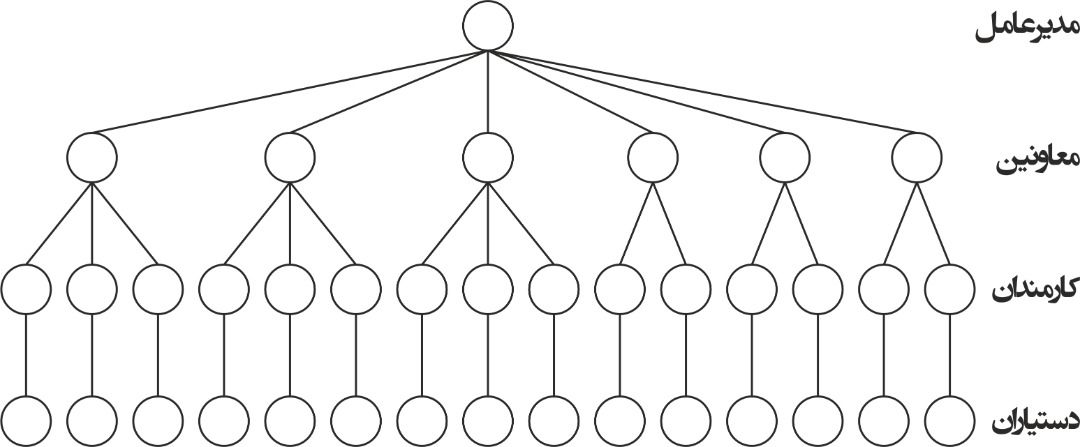
\includegraphics[scale=0.2]{1.jpg}
    \end{center}
    
    حال روی حضور یا عدم حضور مدیرعامل حالت بندی می‌کنیم.(کسانی که حضور دارند را با رنگ سبز و کسانی که حضور ندارند را با رنگ قرمز نشان می‌دهیم)
    
    \textbf{مدیرعامل حضور داشته باشد:} در این صورت هیچ کدام از معاونین نمی‌توانند در مهمانی حضور داشته باشند و ساختار شکل زیر را خواهیم داشت.
    \begin{center}
    	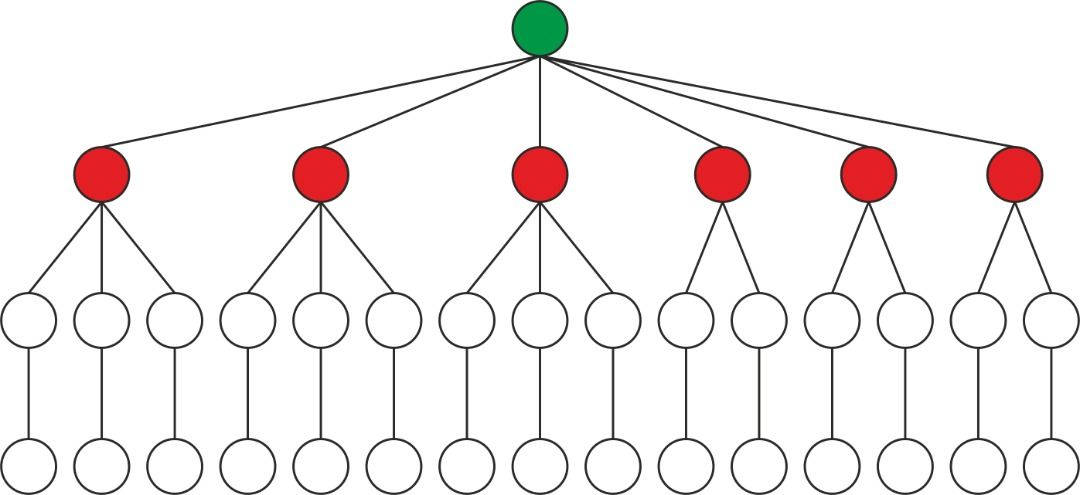
\includegraphics[scale=0.2]{2.jpg}
    \end{center}
    
    حال باید برای هر کدام از جفت‌های کارمند و دستیار، حالات ممکن را به دست بیاوریم. این حالات در شکل زیر نشان داده شده‌اند:
    \begin{center}
    	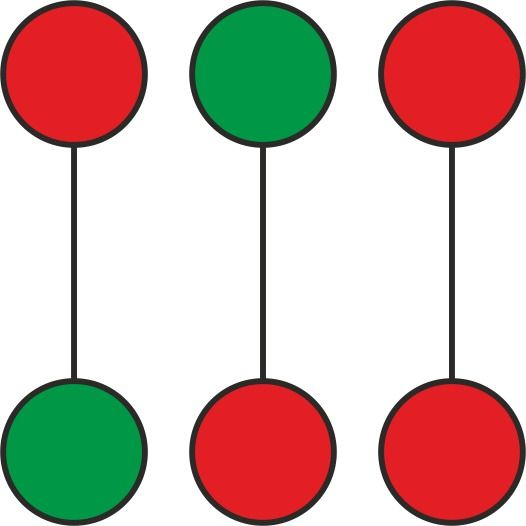
\includegraphics[scale=0.1]{3.jpg}
    \end{center}
    
    پس برای هر کدام از جفت‌ها که از هم مستقل هستند، سه حالت داریم که به یعنی طبق اصل ضرب $3^{15}$ حالت می‌توانیم داشته باشیم.
    
    \textbf{مدیرعامل حضور نداشته باشد:} در این صورت ساختاری شبیه شکل زیر خواهیم داشت. از آنجایی که سه بخش از شرکت 7 نفر و سه بخش دیگر 5 نفر عضو دارد که از یکدیگر مستقل هستند. پس طبق اصل ضرب تعداد  حالات آن‌ها در یکدیگر ضرب می‌شود.
    \begin{center}
    	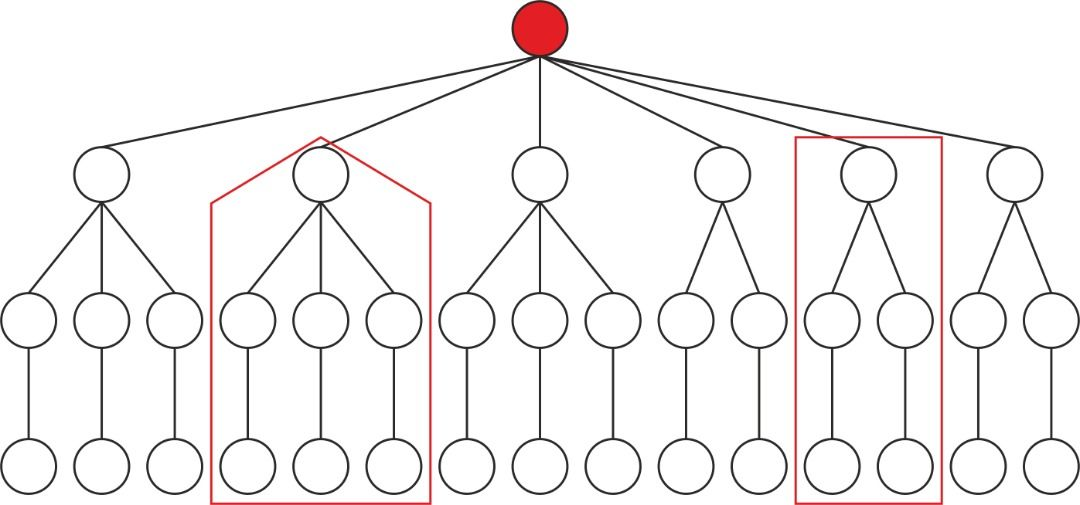
\includegraphics[scale=0.2]{4.jpg}
    \end{center}
    
    \textbf{بخش‌های 7 نفره}: روی حضور یا عدم حضور معاون بخش حالت‌بندی می‌کنیم. اگر در مهمانی حاضر نباشد، سه جفت کارمند و دستیار خواهیم داشت که در مجموع همانند قبل $3^3$ حالت دارند.
    \begin{center}
    	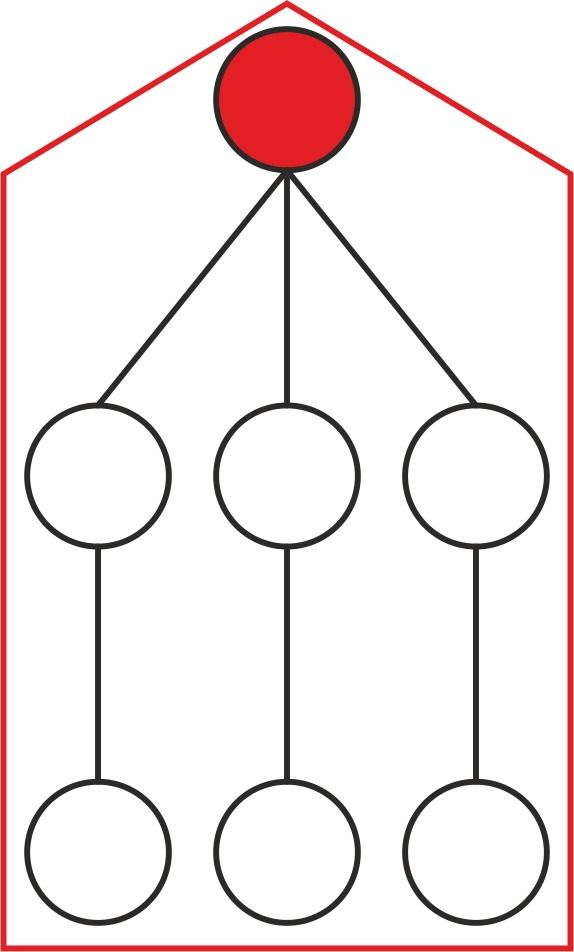
\includegraphics[scale=0.1]{5.jpg}
    \end{center}
    
    اگر معاون بخش در مهمانی حضور داشته باشد، کارمندان او نباید حضور داشته باشند. حال 3 دستیار مستقل داریم که هر کدام دو حالت دارند، پس طبق اصل ضرب $2^3$ حالت داریم.
    \begin{center}
    	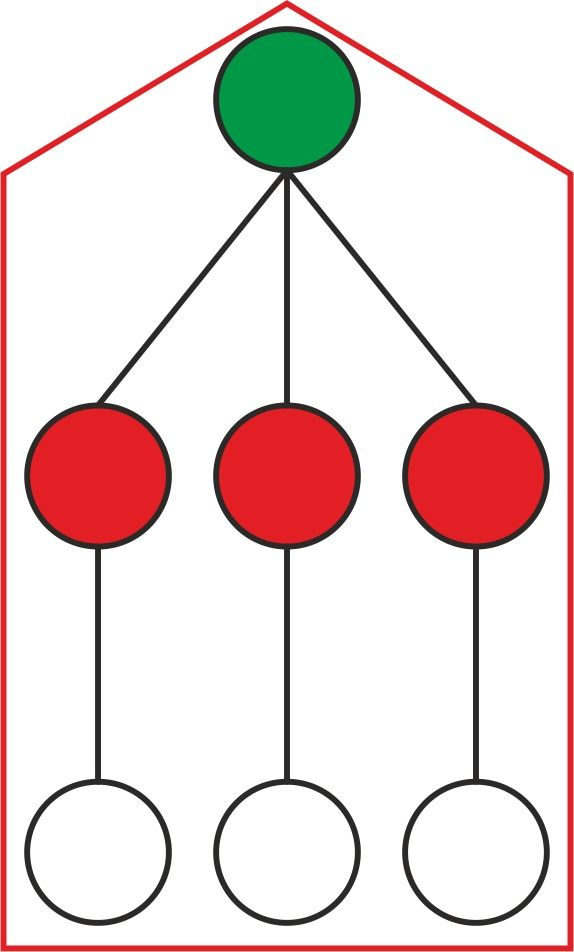
\includegraphics[scale=0.1]{6.jpg}
    \end{center}
    
    پس طبق اصل جمع برای هر بخش 7 نفره شرکت می‌توانیم $3^3 + 2^3 = 35 $ حالت داشته باشیم
    
    \textbf{مجموعه 5 تایی}: روی حضور یا عدم حضور معاون بخش حالت بندی می‌کنیم. اگر در مهمانی حاضر نباشد، دو جفت کارمند و دستیار خواهیم داشت  که در مجموع همانند قبل $3^2$ حالت دارند.
    \begin{center}
    	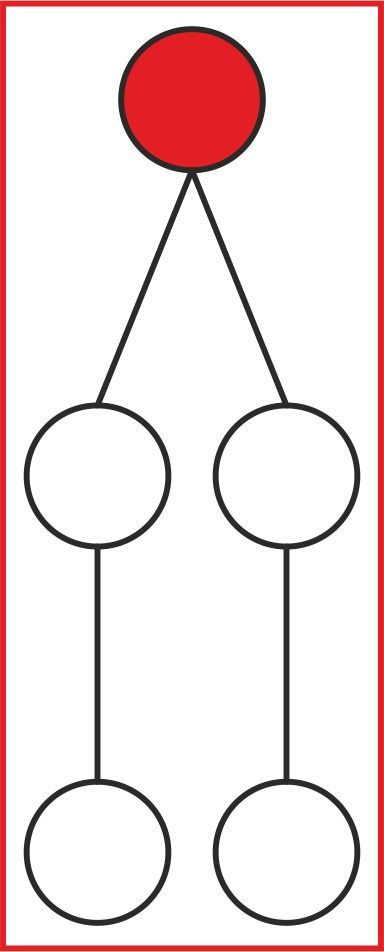
\includegraphics[scale=0.1]{8.jpg}
    \end{center}
    
    اگر معاون بخش در مهمانی حضور داشته باشد، کارمندان او نباید حضور داشته باشند. حال 2 دستیار مستقل داریم که هر کدام دو حالت دارند، پس طبق اصل ضرب $2^2$ حالت داریم.
    \begin{center}
    	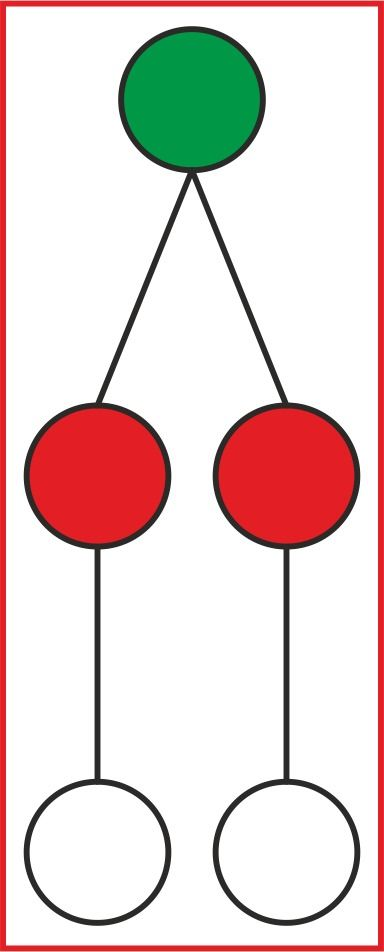
\includegraphics[scale=0.1]{7.jpg}
    \end{center}
    
    پس طبق اصل جمع برای هر بخش 5 نفره شرکت می‌توانیم $ 3^2 + 2^2 = 13 $ حالت داشته باشیم.
    
    و طبق اصل ضرب اگر مدیرعامل شرکت در مهمانی حضور نداشته باشد $ 13^3 \times  35 ^ 3 $ حالت برای برگزاری مهمانی خواهیم داشت.
    
    حال طبق اصل جمع باید حالات به دست آمده در حضور و عدم حضور مدیرعامل را با یکدیگر جمع کنیم:   
    $\mathbf{ 13^3 \times  35 ^ 3  + 3^{15} }$
